% Start of code
\usetikzlibrary{arrows}
\usetikzlibrary{shapes}
% Start of code
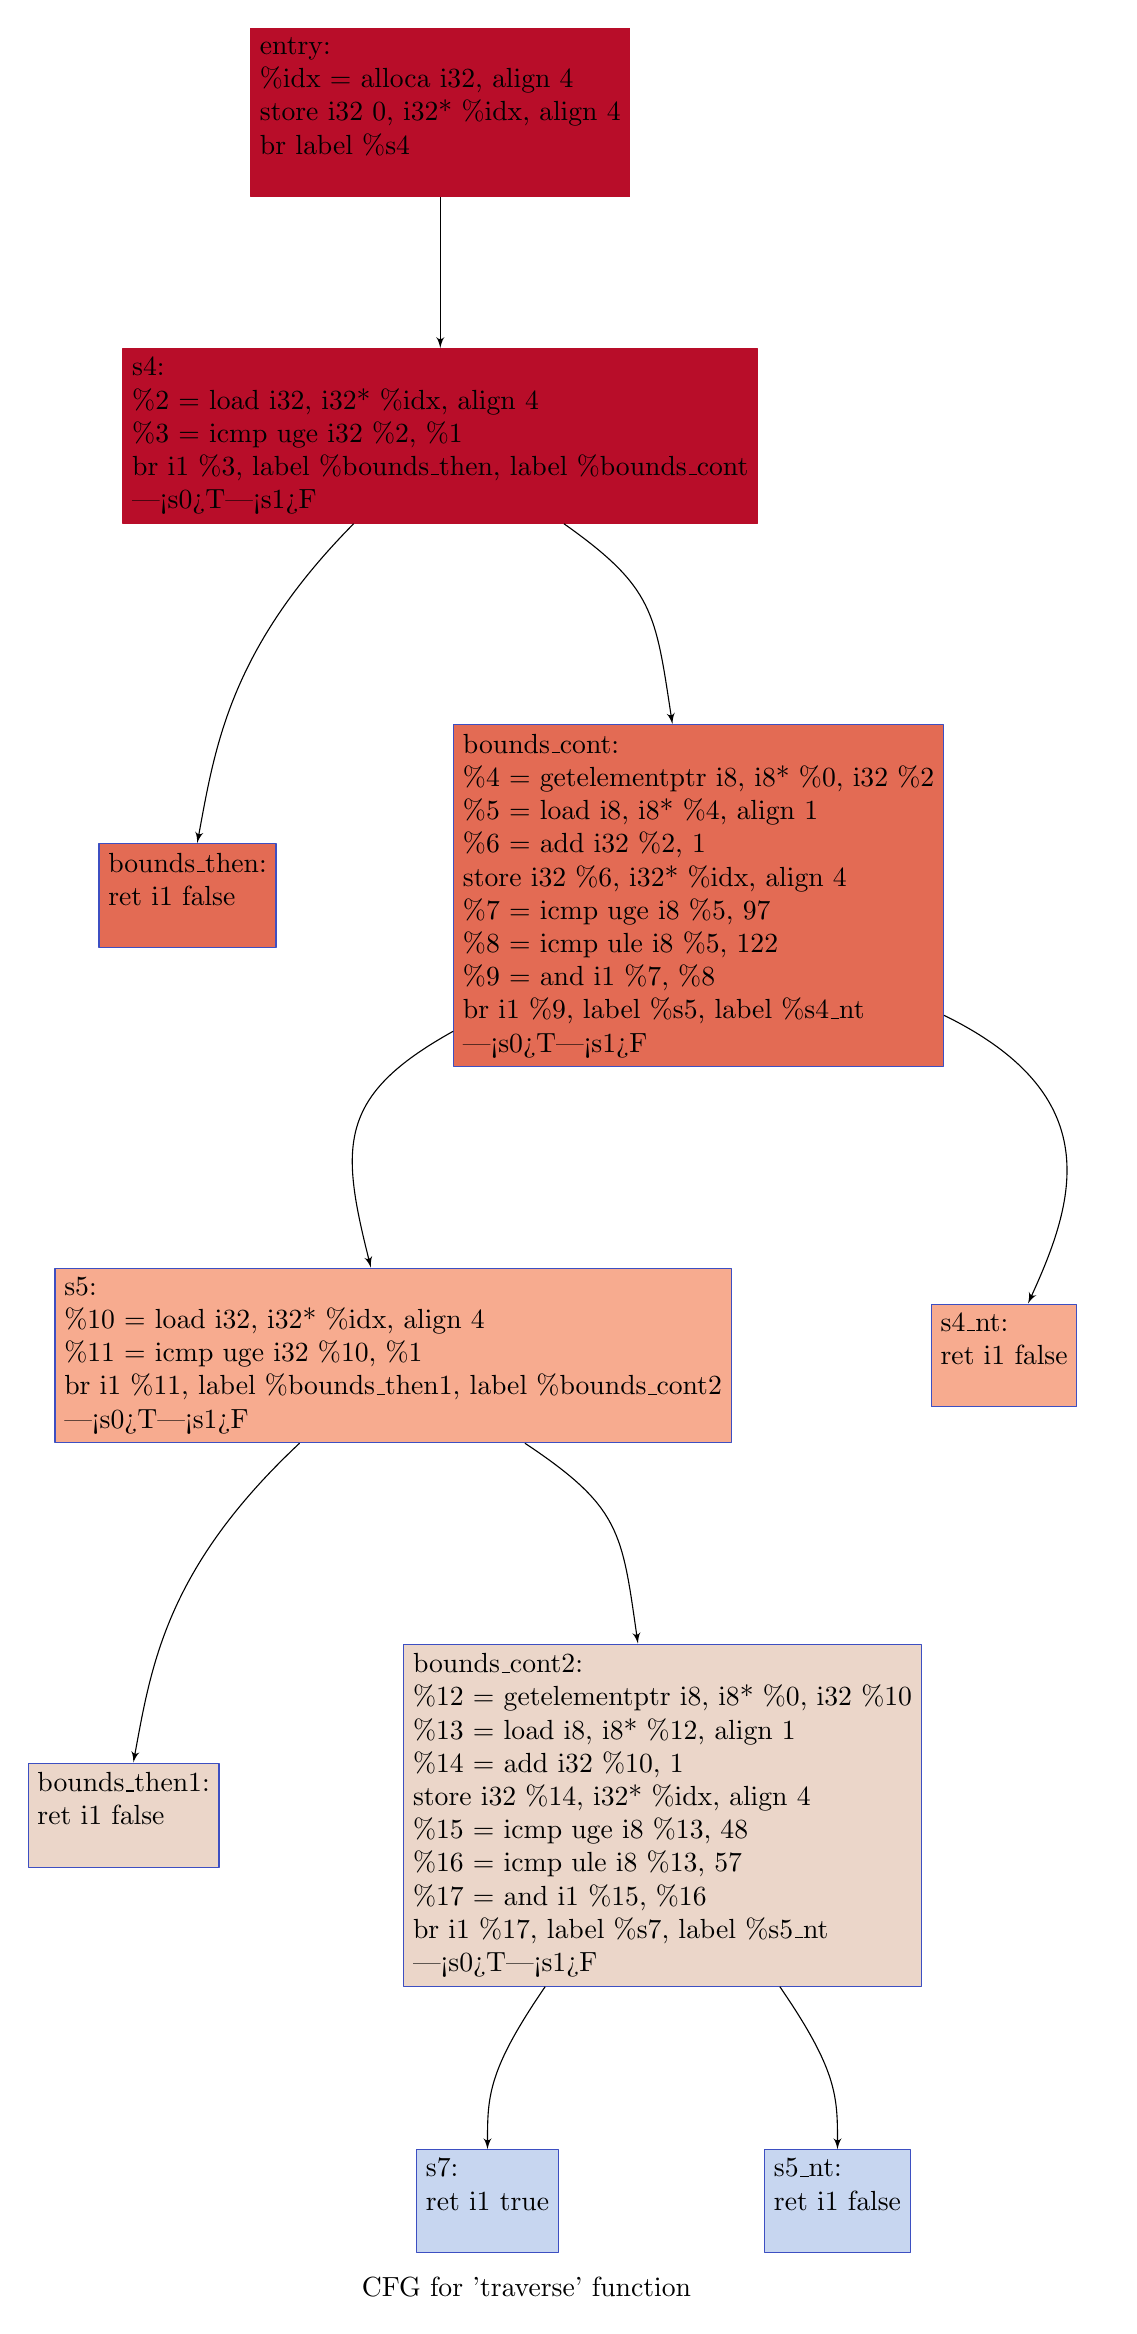
\begin{tikzpicture}[>=latex',line join=bevel]
%%
\begin{scope}
  \definecolor{strokecol}{rgb}{0.0,0.0,0.0};
  \pgfsetstrokecolor{strokecol}
  \draw (211.0bp,11.5bp) node {CFG for 'traverse' function};
\end{scope}
  \definecolor{strokecolor}{rgb}{0.72,0.05,0.16};
  \definecolor{fillcolor}{rgb}{0.72,0.05,0.16};
  \node (Node0x600000748b00) at (180.0bp,794.5bp) [draw=strokecolor,fill=fillcolor,rectangle,align=left] {entry:\\  \%idx = alloca i32, align 4\\  store i32 0, i32* \%idx, align 4\\  br label \%s4\\};
  \definecolor{strokecolor}{rgb}{0.72,0.05,0.16};
  \definecolor{fillcolor}{rgb}{0.72,0.05,0.16};
  \node (Node0x600000748b40) at (180.0bp,678.0bp) [draw=strokecolor,fill=fillcolor,rectangle,align=left] {s4:                                               \\  \%2 = load i32, i32* \%idx, align 4\\  \%3 = icmp uge i32 \%2, \%1\\  br i1 \%3, label \%bounds\_then, label \%bounds\_cont\\|<s0>T|<s1>F};
  \definecolor{strokecolor}{rgb}{0.24,0.31,0.76};
  \definecolor{fillcolor}{rgb}{0.89,0.42,0.33};
  \node (Node0x600000748b80) at (89.0bp,512.5bp) [draw=strokecolor,fill=fillcolor,rectangle,align=left] {bounds\_then:                                      \\  ret i1 false\\};
  \definecolor{strokecolor}{rgb}{0.24,0.31,0.76};
  \definecolor{fillcolor}{rgb}{0.89,0.42,0.33};
  \node (Node0x600000748bc0) at (273.0bp,512.5bp) [draw=strokecolor,fill=fillcolor,rectangle,align=left] {bounds\_cont:                                      \\  \%4 = getelementptr i8, i8* \%0, i32 \%2\\  \%5 = load i8, i8* \%4, align 1\\  \%6 = add i32 \%2, 1\\  store i32 \%6, i32* \%idx, align 4\\  \%7 = icmp uge i8 \%5, 97\\  \%8 = icmp ule i8 \%5, 122\\  \%9 = and i1 \%7, \%8\\  br i1 \%9, label \%s5, label \%s4\_nt\\|<s0>T|<s1>F};
  \definecolor{strokecolor}{rgb}{0.24,0.31,0.76};
  \definecolor{fillcolor}{rgb}{0.97,0.67,0.56};
  \node (Node0x600000748c00) at (163.0bp,347.0bp) [draw=strokecolor,fill=fillcolor,rectangle,align=left] {s5:                                               \\  \%10 = load i32, i32* \%idx, align 4\\  \%11 = icmp uge i32 \%10, \%1\\  br i1 \%11, label \%bounds\_then1, label \%bounds\_cont2\\|<s0>T|<s1>F};
  \definecolor{strokecolor}{rgb}{0.24,0.31,0.76};
  \definecolor{fillcolor}{rgb}{0.97,0.67,0.56};
  \node (Node0x600000748c40) at (383.0bp,347.0bp) [draw=strokecolor,fill=fillcolor,rectangle,align=left] {s4\_nt:                                            \\  ret i1 false\\};
  \definecolor{strokecolor}{rgb}{0.24,0.31,0.76};
  \definecolor{fillcolor}{rgb}{0.92,0.84,0.79};
  \node (Node0x600000748c80) at (66.0bp,181.5bp) [draw=strokecolor,fill=fillcolor,rectangle,align=left] {bounds\_then1:                                     \\  ret i1 false\\};
  \definecolor{strokecolor}{rgb}{0.24,0.31,0.76};
  \definecolor{fillcolor}{rgb}{0.92,0.84,0.79};
  \node (Node0x600000748cc0) at (260.0bp,181.5bp) [draw=strokecolor,fill=fillcolor,rectangle,align=left] {bounds\_cont2:                                     \\  \%12 = getelementptr i8, i8* \%0, i32 \%10\\  \%13 = load i8, i8* \%12, align 1\\  \%14 = add i32 \%10, 1\\  store i32 \%14, i32* \%idx, align 4\\  \%15 = icmp uge i8 \%13, 48\\  \%16 = icmp ule i8 \%13, 57\\  \%17 = and i1 \%15, \%16\\  br i1 \%17, label \%s7, label \%s5\_nt\\|<s0>T|<s1>F};
  \definecolor{strokecolor}{rgb}{0.24,0.31,0.76};
  \definecolor{fillcolor}{rgb}{0.78,0.84,0.94};
  \node (Node0x600000748d00) at (197.0bp,42.5bp) [draw=strokecolor,fill=fillcolor,rectangle,align=left] {s7:                                               \\  ret i1 true\\};
  \definecolor{strokecolor}{rgb}{0.24,0.31,0.76};
  \definecolor{fillcolor}{rgb}{0.78,0.84,0.94};
  \node (Node0x600000748d40) at (323.0bp,42.5bp) [draw=strokecolor,fill=fillcolor,rectangle,align=left] {s5\_nt:                                            \\  ret i1 false\\};
  \draw [->] (Node0x600000748b00) ..controls (180.0bp,752.03bp) and (180.0bp,742.84bp)  .. (Node0x600000748b40);
  \draw [->] (Node0x600000748b40) ..controls (104.0bp,601.07bp) and (98.908bp,565.95bp)  .. (Node0x600000748b80);
  \draw [->] (Node0x600000748b40) ..controls (257.0bp,623.4bp) and (257.42bp,614.49bp)  .. (Node0x600000748bc0);
  \draw [->] (Node0x600000748bc0) ..controls (142.9bp,440.5bp) and (143.93bp,422.61bp)  .. (Node0x600000748c00);
  \draw [->] (Node0x600000748bc0) ..controls (420.47bp,440.5bp) and (408.59bp,402.68bp)  .. (Node0x600000748c40);
  \draw [->] (Node0x600000748c00) ..controls (81.0bp,270.07bp) and (75.908bp,234.95bp)  .. (Node0x600000748c80);
  \draw [->] (Node0x600000748c00) ..controls (245.0bp,292.41bp) and (245.39bp,283.5bp)  .. (Node0x600000748cc0);
  \draw [->] (Node0x600000748cc0) ..controls (197.0bp,89.484bp) and (197.0bp,80.22bp)  .. (Node0x600000748d00);
  \draw [->] (Node0x600000748cc0) ..controls (323.0bp,89.484bp) and (323.0bp,80.22bp)  .. (Node0x600000748d40);
%
\end{tikzpicture}
% End of code
